\documentclass[a4, oneside, 10pt, nobib]{memoir}

%% IMPORTS
% Clickable ref
\usepackage{hyperref}
\usepackage{setspace}
\usepackage{wrapfig}
\usepackage{graphicx}
\usepackage{lipsum}

\usepackage{subcaption}

\usepackage{float}

\usepackage{calc}  
\usepackage{enumitem}

\usepackage{xcolor}
\usepackage{minted}
\usepackage[backend=biber, style=numeric, defernumbers]{biblatex}

%% SET THINGS UP
% Add bibliography database
\addbibresource{bibliography_better.bib}

\definecolor{friendlybg}{HTML}{F8F8F8}

% Minted macros
% Will append "code" to the environment name by default
\newminted{python}{style=friendly, bgcolor=friendlybg, breaklines, tabsize=2}
\newminted{text}{style=friendly, bgcolor=friendlybg, breaklines, tabsize=2, breakanywhere}
\newminted{shell}{style=friendly, bgcolor=friendlybg, breaklines, tabsize=2, breakanywhere}
\newminted{yaml}{style=friendly, bgcolor=friendlybg, breaklines, tabsize=2, breakanywhere}
\newminted{nginx}{style=friendly, bgcolor=friendlybg, breaklines, tabsize=2, breakanywhere}
\newminted{json}{style=friendly, bgcolor=friendlybg, breaklines, tabsize=2, breakanywhere}



\usepackage[xindy, toc, acronyms, nomain]{glossaries}

\usepackage{tikz}
\usetikzlibrary{positioning}

\tikzset{basic/.style={draw,fill=blue!20,text width=1em,text badly centered}}
\tikzset{input/.style={basic,circle}}
\tikzset{weights/.style={basic,rectangle}}
\tikzset{functions/.style={basic,circle,fill=blue!10}}

\newacronym{lvm}{LVM}{Logical Volume Manager}

\makeglossaries


% Tables
\usepackage{multirow}

% micro sign != MU
\usepackage{siunitx}

% Typography
\usepackage{fontspec}
	% Numbers={OldStyle,Proportional},Ligatures=TeX
	\setmainfont[]{Adobe Caslon Pro}
	\setmonofont[Scale=0.75]{Iosevka Etoile}
	%\newfontfamily\bold{Tiempos Headline Medium}

% Captions
\usepackage[font=normalsize, labelfont=bf]{caption}
\captionsetup[table]{position=below}
\captionsetup[figure]{position=below}

% Figures
\graphicspath{ {figures/} }
%\definecolor{gray75}{gray}{0.75}

% Set Table of Contents depth
\setsecnumdepth{subsection}
\settocdepth{subsection}

% Style Abstract (and Acknowledgements)
\renewcommand{\abstractnamefont}{\normalfont\huge\bfseries}
\renewcommand{\abstracttextfont}{\normalfont\normalsize}

% Utilities
\newcommand{\code}{\texttt}

%\settypeblocksize{20cm}{16.5cm}{*}%

%% DOCUMENT
\begin{document}

% Add revision data
\input{revision}

%\setlrmarginsandblock{2.5cm}{2.5cm}{*}
%\setulmarginsandblock{2.5cm}{*}{1}
%\checkandfixthelayout 

% Frontmatter part is numbered with Romans
\frontmatter

% Preamble:
%  Front, Dedication, Abstract and Acknowledgements
% Based on https://github.com/dubvulture/thesis/blob/master/frontispiece.tex

\thispagestyle{empty}

\begin{wrapfigure}{l}[22mm]{0.20\textwidth}
	\vspace*{-8mm}
	\centering
	\includegraphics[width=0.20\textwidth]{logo-bicocca.jpg}
\end{wrapfigure}
\large \noindent \textsc{Università degli Studi di Milano Bicocca} \\
\textbf{Dipartimento di Informatica, Sistemistica e Comunicazione \\
	Corso di Laurea Magistrale in Informatica}

\vfill


\begin{center}
	{\Huge \textbf{Modernising the CERN CMS Trigger Rates Monitoring software}}
\end{center}

\vfill

\begin{flushleft}
	{\Large \textbf{Supervisor:} \textit{Fabio Stella} \\
		\textbf{Co-supervisor:} \textit{Simone Gennai} \\
		\textbf{Co-supervisor:} \textit{Glenn Dirkx}}
\end{flushleft}

\vspace{8mm}
\par

\begin{flushright}
	{\Large \textbf{Master Thesis} \\
		\textit{Antonio Vivace} \\ 793509}
\end{flushright}

\vfill
\par

\begin{center}
	{\large Academic Year 2019 -- 2020}

	% Print revision data and WIP notice
	\hfill\linebreak
	Work In Progress Draft (!)

	Revision \texttt{\revision} (\texttt{\revisiondate})

	\url{https://avivace.com/thesis.pdf} for the latest build.
\end{center}

\clearpage
\clearpage
\begin{flushright}
	\thispagestyle{empty}
	\vspace*{50 mm}
	To \textit{Mene}, the scientist of the family.

\end{flushright}
\clearpage
\phantomsection
\addcontentsline{toc}{chapter}{Abstract}

\begin{vplace}[0.7]
	\renewcommand*\abstractname{Abstract}

	\begin{abstract}

		\fontsize{11}{12}\selectfont\baselineskip=1.2em

		High Energy Physics experiments involve large amount of complex systems subject to anomalies and malfunctioning. They generate a lot of high dimensional and contextual data that must be monitored and analysed by a Data Quality Monitoring team to validate and deliver certified data for physics analysis.

		At the European Organization for Nuclear Research (CERN), in the Large Hadron Collider (LHC), the Compact Muon Solenoid (CMS) experiment generates events at a rate of 40 MHz, each one carrying payloads averaging 1.5 MB. It is the job of the Trigger System to discard the large majority of this data and retain the most interesting one.

		This crucial phase is sensible to malfunctions of many of the underlying parts, from sub detectors to the trigger algorithms configurations.

		Shifters in the CMS Control Room use a Rate Monitoring software to monitor Trigger Rates and spot potential problems by looking at reference fits and other detector diagnostic data.

		We proceed to improve and renovate this software, exploiting the new features to integrate the Trigger data with another dataset from the new CMS Run Registry, describing the status over time of every part of the detector, including the ones for which the failures are identifiable from the monitoring of the trigger rates.

		The resulting dataset can potentially aid novel Anomaly Detection approaches to this challenge.

		\normalsize

	\end{abstract}

\end{vplace}

\thispagestyle{empty}

\pagebreak
\phantomsection
\addcontentsline{toc}{chapter}{Acknowledgements}

\renewcommand*\abstractname{Acknowledgements}

\begin{vplace}[0.7]

	\begin{abstract}

		\fontsize{11}{12}\selectfont\baselineskip=1.2em

		I would like to express my appreciation to Simone Gennai, Fabio Stella, Pietro Govoni and Glenn Dirkx, for giving me the chance to work on a project of this incredible magnitude, joining a unique community of passionate researchers. Furthermore, they gave me the freedom, the tools and the motivations to investigate my ideas, while also being critical and providing invaluable feedback.

		I extend my gratitude to everyone at CERN who gave me useful advices and precious insights: Dinyar Rabady, Andrea Bocci, Fabio Espinosa, Adrian Alan Pol, Alessandro Thea and Sam James Harper.

		Thanks to CERN and the CMS collaboration for providing the funds, the datasets and the computing resources used in this work.

		At my home university, I would like to mention Leonardo Mariani, Daniela Micucci, Edoardo Datteri and Roberto Previtera. I also thank the students I supervised, Riccardo, Alessandro, Morris, Luca and Stefano, from whom I learned a lot.

		I send my love to the inspiring and brilliant teachers I had during my earlier education: Camilla D'Andria, Caterina Brasacchio, Maurizia Perego, Luca Mauri.

		Thanks to my friends in Italy and France, too many to name them all, for keeping me sane, loved and happy.

		Last, but definitely not least, my family has been essential and I can't express how grateful I am for the support, the unconditional love and the appreciation with which they always enabled my passions and promoted my choices.

	\end{abstract}

\end{vplace}

\thispagestyle{empty}



\pagebreak

% Table of Contents (hidden from the table of contents)
\tableofcontents*
\thispagestyle{empty}

% Switch to Arabic numbering with mainmatter
\mainmatter

% Include chapters
\chapter{Introduction}

\section{Motivations}

\paragraph{Monitoring a a particle detector} The CMS detector at the LHC particle accelerator is a complex system which needs fast and reliable monitoring. Quick feedback on each of the subsystems is needed to spot and solve problems or the data taken might not be useful for physics analysis \cite{chep2016wbm}. Experts from different systems need to correlate information to investigate underlying problems.

A centralized monitoring solution exposes real time data, historical information, summaries and reports from a series of different sources:

\begin{itemize}
	\item Luminosity, Collision Rates.
	\item Global Trigger, \textbf{Trigger Rates}.
	\item LHC (Beam currents, losses, status, collimators, real time clock, event signal).
	\item Magnet.
	\item Sub-system specific information stored in relational databases.
	\item DAQ.
	\item DQM.
	\item Experimental running conditions in database.
	\item Hardware.
	\item Other non event data.
\end{itemize}

Such system is different from the Data Quality Monitoring service, which look at actual \textit{event} data.

The WBM software covered this role since the commissioning of the CMS experiment (2008), evolving and integrating new services into a growing framework during LHC Run 1 (2010-2013) and Run 2 (2015-2018).

\paragraph{Upgrading the monitoring framework} 

During the second Long Shutdown of the LHC (2018-2021) the CMS detector will be upgraded and many CMS sub-systems will drastically change. WBM started to show its age and problems: it unexpectedly and heavily grew with new features, arriving at a point where services were using vastly different technologies and it became harder and harder to maintain and expand \cite{CMSWBMreview}. It has been decided to deprecate \cite{upgradewbmoms} WBM in favour of a new software framework, called OMS, decoupling the UI from the Aggregation (Data) Layer.

\paragraph{Monitoring the Trigger System}

This work concerns one of the sources of monitored data: RateMon, the software providing Trigger Rates data, querying the OMDS database and carrying out \textbf{normalisations} and \textbf{corrections} for a number of different configurations and conditions, allowing consistent comparisons.

The Trigger system is responsible of filtering the large majority of events, spotting the potentially interesting ones, triggering the detector's read-out system to actually record data from the selected collisions. Monitoring the rates of such filters is essential to spot any anomalous behaviour in the underlying (sub)systems, software and/or hardware configurations, network and detector malfunctions.

Trigger Rates are presented in the form of \textit{Rates VS PU} \textbf{plots}. It also responsible of \textbf{alerting} the Trigger Shifters staff when recorded rates deviate too much from the \textbf{predicted} values. Those predictions are based on analytical models fitted on data collected in previous runs.

\section{Scope}

Two main tasks have been carried out during this experience:

\paragraph{Development and study of the Rate Monitoring Software} TODO

\paragraph{Experimental Anomaly Detection approaches} TODO


\section{Structure}

We will start by introducing CERN in Chapter \ref{background}, the research institute operating the LHC, briefly describing its relevance and its achievements in science, software and computing, besides its major commitment in fundamental research.

To justify the motivations and the unique magnitude of the Large Hadron Collider particle accelerator, some basics notions and concepts in Particle Physics are explained and contextualised. In particular, how statistics plays a vital role in this research field, providing some of the main tools to validate theories. A brief description of LHC and the CMS detector follows, explaining some of the jargon used in this domain, essential to understand the context of our work.

Finally, some background on Anomaly Detection and Machine Learning is given, surveying some applications and recent papers.

Chapter \ref{ratemon} gives a detailed report of the context, the research and development work done on the Rate Monitoring tools, outlining the achieved results and how they improve the user experience and enable new features and possibilities.

In chapter \ref{dataset} we introduce some Anomaly Detection applications to similar challenges at CERN, evaluating their results and practical effects to the current workflows. One of the common problems in such attempts is the inherent difficulty to obtain usable datasets encompassing enough features to encode the phenomena and the contextual knowledge and data considered in the current pipelines.

We exploit the acquired knowledge and the new developed features on the Rate Monitoring software to tackle exactly this issue: we integrate Trigger Rates data with another dataset, (hopefully) providing a new starting point to enable future experimentations on this matter.


\section{Conventions}

Implementation work on existing software was done trough Merge Requests to the main codebase. Each described task is accompanied with a corresponding sitography entry.

Code snippets (called "listings", from now on) demonstrating the execution of commands in a shell are noted with the \mcode{\$} character. Preceding the \mcode{\$} character you sometimes notice a string specifying the hostname of the machine (as specified in CERN OpenStack) or the general infrastructure/service in which that commands must run to have effect. E.g. \mcode{lxplus \$ command} shows the command execution on one of the machine from LXPLUS \cite{LXPLUSServiceITDepartment-2020-10-01}, the CERN service offering access to machines running Linux CERN CentOS 7. If there's no specification before \mcode{\$}, the environment is not relevant. With \mcode{P5} we refer to the machines installed in Point 5 of the LHC, in Cessy (France), home to the CMS detector.

The produced source code has been reported here only partially, focusing only on the relevant and meaningful parts. Refer to the git repositories for the complete copies. Some listings also have truncated outputs for the same reasons.
\section{Anomaly Detection}

In data mining, \textit{Anomaly Detection} is a classification problem: the goal is finding patterns in data that do not conform to expected behavior \cite{chandola2009anomaly}. These patterns often denote an underlying different process: an anomaly can be defined an observation which deviates so much from the other observations as to arouse suspicions that it was generated by a different mechanism \cite{hawkins1980identification}.

This task finds extensive use in many domains, such as fraud detection for credit cards, insurance or health care, intrusion detection for cyber security, military surveillance and fault detection in critical systems.

Anomalies are also referred to as outliers, novelties, deviations, exceptions or noise. \textit{Noise removal} and \textit{noise accomodation} are related problems, dealing with the removal of unwanted objects before performing data analysis (removal) and immunizing a statistical model against anomalous observations (accomodation).

Methods make use of tools and concepts from a number of different fields, such as machine learning, data mining, information theory, spectral theory and statistics.

\subsection{Challenges}

Anomaly detection is an hard and complex problem, mainly due to the following challenging factors:

\begin{enumerate}
	\item Defining the normal and anomalous regions and their boundaries;
	\item The notion of \textit{normality} may evolve with time;
	\item Anomalies may be different for different domains; A small fluctuation might be significant in one domain while being a normal in another one;
	\item Availability of labeled data;
	\item Noisy data and anomalies can be hard to discriminate.
\end{enumerate}

To justify the variety of strategies and techniques and show the breadth of problem domain, we will outline the several factors determining an Anomaly Detection problem.

\subsection{Nature of data}

The input is usually a collection of data instances (record, event, observation), described by one (univariate) or more (multivariate) attributes (feature, variable). Each attribute can be of different types (binary, categorical, continuos).

\subsection{Type of Anomaly}

\begin{enumerate}
	\item Point Anomalies
	\item Contextual Anomalies
	\item Collective Anomalies
\end{enumerate}


\subsection{Data labels}

The information associated with a data instance, describing if the instance is normal or anomalous is called label.


\subsubsection{Supervised}
\subsubsection{Semi-supervised}
\subsubsection{Unsupervised}

\subsubsection{Evaluation}

Here, we introduce some classification performance metrics used to set up a formal procedure to evaluate different approaches.

\begin{table}[]
	\centering
	\begin{tabular}{lllll}
		                                     &          &                                           &          & \\
		\multirow{2}{*}{}                    &          & \multicolumn{2}{l}{\textbf{Ground Truth}} &            \\
		                                     &          & Positive                                  & Negative & \\
		\multirow{2}{*}{\textbf{Prediction}} & Positive & TP                                        & FP       & \\
		                                     & Negative & FN                                        & TN       &
	\end{tabular}
	\caption{Confusion Matrix}
	\label{table:confusion_matrix}
\end{table}

Table \ref{table:confusion_matrix} explains the following quantities:

\begin{itemize}
	\item TP True Positives
	\item FP False Positives
	\item FN False Negatives
	\item TN True Negatives
\end{itemize}

Receiver Operating Characteristics (ROC) diagrams show a classifier performance plotting the False Positive Rates (FPR) against the True Positive Rates (TPR) of the classifier for a different thresholds. The idea is maximise the area under the ROC curve.

Intuitively, precision is the ability of the classifier not to label as positive a sample that is negative while recall is a measure of the ability of the classifier to find all the positive samples. \cite{scikit-learn}


\begin{equation}
	TPR = Recall = r = \frac{TP}{TP+FN}
\end{equation}

\begin{equation}
	FPR = \frac{FP}{FP+TN}
\end{equation}

\begin{equation}
	Precision = p = \frac{TP}{TP+FP}
\end{equation}

Another metric is the F-measure, defined as follows:

\begin{equation}
	F_\beta = (1 + \beta^2) \cdot \frac{\mathrm{p} \cdot \mathrm{r}}{(\beta^2 \cdot \mathrm{p}) + \mathrm{r}}
\end{equation}

Where $\beta$ is a positive real chosen such that recall is considered $\beta$ times as important as precision. In the case $\beta = 1$:

\begin{equation}
	F_1 = 2 \cdot \frac{\mathrm{p} \cdot \mathrm{r}}{\mathrm{p} + \mathrm{r}}
\end{equation}



\subsection{Output of Anomaly Detection}

\subsection{Applications}



\chapter{Machine Learning}

\section{Artificial Neural Networks}

\textit{Artificial Neural Networks} are mathematical models inspired by biological neural networks. They are composed of (layers of) connected neurons and characterized by processes changing their structure based on the flowing information during the \textit{learning} stage.

The first mention of this term is in McCulloch and Pitts' 1943 work \cite{McCulloch1943}, where they introduced a Threshold Logic Unit (or Linear Threshold Unit), able to implement simple boolean functions \ref{fig:TLU}.

\begin{figure}[H]
	\centering
	\begin{equation*}
		\begin{aligned}[c]
			TLU(\vec{x}) & = \phi \bigg( \sum_{i=1}^{n}{w_{i} \cdot x_{i}} \bigg) \\
			\phi(x)      & = x - \theta \geq 0
		\end{aligned}
		\quad
		\begin{aligned}[c]
			n      & = 2   \\
			\theta & = 1.5 \\
		\end{aligned}
		\quad
		\begin{aligned}[c]
			w_{1} & = 1.0 \\
			w_{2} & = 1.0
		\end{aligned}
	\end{equation*}
	\caption{Boolean logic AND implemented by a Threshold Logic Unit}
	\label{fig:TLU}
\end{figure}

\paragraph{Perceptron}

Rosenblatt introduced in 1958 the \textit{Perceptron}\cite{rosenblatt1958perceptron}, a linear binary classificator now considered the simplest feed-forward neural network.

It can be modeled as follows:

\begin{equation*}
	\begin{aligned}[c]
		f(\mathbf{x}) = \begin{cases}1 & \text{if }\ \mathbf{w} \cdot \mathbf{x} + b > 0,\\0 & \text{otherwise}\end{cases}
	\end{aligned}
\end{equation*}

\begin{equation*}
	\begin{aligned}[c]
		w = \begin{bmatrix}
			w_{1} & \cdots & w_{d} & b
		\end{bmatrix}
	\end{aligned}
	\quad
	\begin{aligned}[c]
		\vec{x} = \begin{bmatrix}
			x_{1}  \\
			\vdots \\
			x_{d}  \\
			1
		\end{bmatrix}
	\end{aligned}
\end{equation*}

\begin{figure}[H]
	\centering
	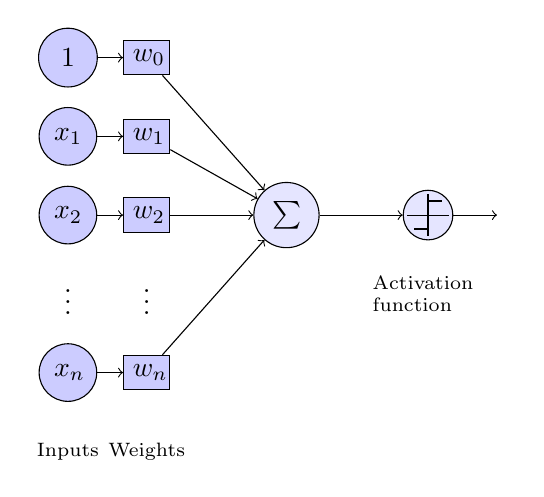
\begin{tikzpicture}
		\node[functions] (center) {};
		\node[below of=center,font=\scriptsize,text width=4em] {Activation function};
		\draw[thick] (0.5em,0.5em) -- (0,0.5em) -- (0,-0.5em) -- (-0.5em,-0.5em);
		\draw (0em,0.75em) -- (0em,-0.75em);
		\draw (0.75em,0em) -- (-0.75em,0em);
		\node[right of=center] (right) {};
		\path[draw,->] (center) -- (right);
		\node[functions,left=3em of center] (left) {$\sum$};
		\path[draw,->] (left) -- (center);
		\node[weights,left=3em of left] (2) {$w_2$} -- (2) node[input,left of=2] (l2) {$x_2$};
		\path[draw,->] (l2) -- (2);
		\path[draw,->] (2) -- (left);
		\node[below of=2] (dots) {$\vdots$} -- (dots) node[left of=dots] (ldots) {$\vdots$};
		\node[weights,below of=dots] (n) {$w_n$} -- (n) node[input,left of=n] (ln) {$x_n$};
		\path[draw,->] (ln) -- (n);
		\path[draw,->] (n) -- (left);
		\node[weights,above of=2] (1) {$w_1$} -- (1) node[input,left of=1] (l1) {$x_1$};
		\path[draw,->] (l1) -- (1);
		\path[draw,->] (1) -- (left);
		\node[weights,above of=1] (0) {$w_0$} -- (0) node[input,left of=0] (l0) {$1$};
		\path[draw,->] (l0) -- (0);
		\path[draw,->] (0) -- (left);
		\node[below of=ln,font=\scriptsize] {Inputs};
		\node[below of=n,font=\scriptsize] {Weights};
	\end{tikzpicture}
\end{figure}

\subsection{Activation Functions}
\begin{description}[leftmargin=!,labelwidth=\widthof{\bfseries The longest label}]
	\item[Logistic]
	      ${(1 + e^{-x})}^{-1}$
	\item[Hyperbolic]
	      $\tanh(x)$
	\item[Rectified Linear Unit (ReLU)]
	      $\max(0,\, x)$
	\item[Leaky ReLU]
	      $\max(0.01x,\, x)$
	\item[Parametric LReLU]
	      $\begin{cases}
			      \alpha x & \text{if } x \geq 0 \\
			      x        & \text{if } x < 0    \\
		      \end{cases}$
	\item[Exponential Linear Unit (ELU)]
	      $\begin{cases}
			      \alpha(e^x - 1) & \text{if } x \geq 0 \\
			      x               & \text{if } x < 0    \\
		      \end{cases}$
\end{description}

\begin{figure}
	\centerline{
		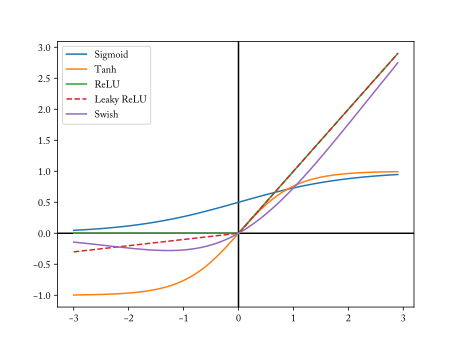
\includegraphics[width=0.4\paperwidth]{activation_fun_comparison}}
	\caption{Comparison of activation functions}
	\label{fig:activation_functions}
\end{figure}

\chapter{Modernising Rate Monitoring Tools}

This chapter gives an overview of the software development work done to improve and add new features to the CMS Rate Monitoring software. Some other experimental components have ben developed to showcase possible upgrades, delivering quality of life enhancements and enabling shifters and physicists to navigate data in a faster and more comfortable way. This work is also described in \cite{VivaceRTM1} \cite{VivaceRTM2} \cite{L1TriggerOMSDevelopments} \cite{MohrmanRTM} and the code is available in the mentioned git repositories.

\begin{figure}
	\centerline{
		\includegraphics[width=0.6\paperwidth]{figures/RMT_305112_L1_SingleTau120er2p1.pdf}}
	\caption{L1 Trigger path plotted with a fitted function on run 305112}
	\label{fig:ratemon_l1}
\end{figure}

\begin{figure}
	\centerline{
		\includegraphics[width=0.6\paperwidth]{figures/RMT_305112_HLT_PFMET110_PFMHT110_IDTight.pdf}}
	\caption{HLT Trigger path plotted with a fitted function on run 305112}
	\label{fig:ratemon_hlt}
\end{figure}


\section{Context}

What are ratemon scripts? How are they used? By whom?

\subsection{ShiftMonitorTool}

The High Level Trigger (HLT) rate monitoring tool is a python script that reports the rates of a selected list of triggers, primary datasets, and streams. The script updates every minute and averages the rates recorded in the last 3 lumisections, and, if possible, compares them to the predicted rate. If a trigger path deviates by a specified amount from the prediction, or exceeds a fixed rate, the corresponding line is highlighted in a yellow colour. The scripts also displays other information that could be useful for the shifter, such as the run number and last lumisections, the LHC status, HLT key, deaditme, instantaneous luminosity and index of the prescale column in use.

\begin{figure}
	\centerline{
		\includegraphics[width=0.8\paperwidth]{figures/ratemon_warnings}}
	\caption{Example execution of the Rate Monitoring Tool showing warnings: two triggers have values consistently deviating from the predictions. \cite{ratemon-twiki}}
	\label{fig:ratemon_warnings}
\end{figure}

\section{Packaging, CI/CD}

To enable CI/CD, we copied the repository on the CERN GitLab. The repository on GitHub is being kept updated but the CI/CD is handled by GitLab.
I've restructured the folder. The "misc" folder now contains the fits logs and the wbmRateReader. The ratemon folder is the only one actually being packaged. The "systemd" folder contains the service file allowing the \texttt{ShiftMonitorTool} to be installed and used as a systemd service.

Docker, GitLab ci, cernbox

Each commit triggers a build and a deployment of a RPM package. This CI/CD system is configured in these files:

\begin{enumerate}
	\item \texttt{.GitLab-ci.yml} - describes the GitLab CI. The first phase (\texttt{build\_rpm}) tells the builder (described by \texttt{builder.dockerfile} and exposed on the GitLab registry) to run \texttt{make rpm} (described in \texttt{Makefile}) and flags the RPM package files as artifacts; In the second phase (deploy), those artifacts are pushed on a EOS folder using the ci-web-deployer tool;
	\item builder.dockerfile - prepares the docker container that will run the build, starting from the cern/cc7-base image. This is exposed using the GitLab registry feature as gitlab-registry.cern.ch/avivace/ratemon/builder;
	\item Makefile - Uses the fpm tool to produce an RPM file with the given metadata and contents. Basically, the ratemon script folder is copied into /opt/ and the systemd service file goes into /usr/lib/systemd/system

	\item The build produces an RPM package file. Those files are pushed during the "deploy" CI phase and finally published on a public CERNBox folder (EOS: /eos/users/a/avivace/ratemon\_builds). This is done using a service CERN account.
\end{enumerate}

Previously, the RateMon tools had to be installed checking out the code from the git repository, running a preparatory script, configuring the database connection and then running the script. Now, the system package manager can install the packaged software.

\section{Configuration}

YAML, schema, database errors?

The ShiftMonitorTool and plotTriggerRates scripts now require an \texttt{--dbConfigFile} option, specifying the YAML configuration file containing the database connection parameters.

I've updated the README and the twiki page to reflect the changes on the DB configuration. Scripts now need to be called in this way:

\texttt{python plotTriggerRates.py --dbConfigFile=dbConfig.yaml --useFills --createFit --bestFit --triggerList=TriggerLists/monitorlist\_COLLISIONS.list 6303}

\section{Exporting data}

JSON, middle db layer?

\section{Python3 upgrade}

TODO

\section{From a CLI tool to a proper module}

TODO

\section{API}

Connexion, OpenAPI 3 schema, Swagger UI
\begin{verbatim}
yum install libnsl

export LD_LIBRARY_PATH=/usr/lib/oracle/19.6/client64/lib:LD_LIBRARY_PATH

copy tnsnames.ora

wget https://download.oracle.com/otn_software/linux/instantclient/19600/oracle-instantclient19.6-basic-19.6.0.0.0-1.x86_64.rpm

yum install oracle-instantclient19.6-basic-19.6.0.0.0-1.x86_64.rpm
\end{verbatim}

\section{Web Application}

VueJS, ROOT, Plotly

\section{Integration with OMS}

Highcharts, React, Panel

\section{Run Registry}

CMS Run Registry is a in-development tool giving access to a lot of DQM datasets. TODO: describe bug reports, HTTPS auth problems and various contributions done upstream to this tool.


\section{Deployment}

\subsection{Attaching a volume for caching}

To offer more disk space to the caching mechanism, a new volume has been created through the CERN Openstack control panel. Once available, I attached it to the machine serving the RateMon API.

On that machine, \texttt{fdisk -l} will give the disks overview, listing the new volume. I noted the device ID (\texttt{/dev/vdb}) and then executed \texttt{fdisk /dev/vdb} to launch fdisk, the partition manager tool provided by the util-linux standard package.

\begin{verbatim}
[root@ater ~]# fdisk -l
...
Disk /dev/vdb: 600 GiB, 644245094400 bytes, 1258291200 sectors
Units: sectors of 1 * 512 = 512 bytes
Sector size (logical/physical): 512 bytes / 512 bytes
I/O size (minimum/optimal): 512 bytes / 512 bytes
\end{verbatim}

In the fdisk shell, create a new partition (\texttt{n}), select is a primary (\texttt{p}) and denote it as the first (\texttt{1}). Set it to occupy all the available space accepting defaults. Select again the partition (\texttt{t}) and set the Linux partition type (\texttt{83}). (\texttt{p}) displays the partition setup we just defined. If that's okay, (\texttt{w}) commits the modifications and applies them.

\begin{verbatim}
Device     Boot Start        End    Sectors  Size Id Type
/dev/vdb1        2048 1258291199 1258289152  600G 83 Linux
\end{verbatim}

Back in the standard shell, use \texttt{mkfs.ext4 /dev/vdb} to format the partition using the EXT4 file system.

Note the UUID of our newly formatted partition:

\begin{verbatim}
[root@ater ~]# mkfs.ext4 /dev/vdb
mke2fs 1.45.4 (23-Sep-2019)
Creating filesystem with 157286400 4k blocks and 39321600 inodes
Filesystem UUID: f74a87c8-7ced-4414-bc62-e09d07be7845
\end{verbatim}

Now that we know the UUID, we can mount the volume:

\begin{verbatim}
[root@ater ~]# mkdir /cache
[root@ater ~]# mount /dev/disk/by-uuid/f74a87c8-7ced-4414-bc62-e09d07be7845 /cache
\end{verbatim}

To make the mounting persistent, we add this entry to the \texttt{/etc/fstab} file:

\begin{verbatim}
UUID=f74a87c8-7ced-4414-bc62-e09d07be7845	/cache	auto defaults,nofail	0 3
\end{verbatim}

Here's the final situation, as described by \texttt{df -h}:

\begin{verbatim}
[root@brandeis ~]# df -h
Filesystem      Size  Used Avail Use% Mounted on
...
/dev/vda2        40G   33G  7.6G  82% /
/dev/vdb        590G   73M  560G   1% /cache
\end{verbatim}

\subsection{NGINX as reverse proxy and cache server}

\begin{verbatim}
sudo cat /var/log/audit/audit.log | grep nginx | grep denied
\end{verbatim}

\begin{verbatim}
[root@ater ~]# setsebool -P httpd_can_network_connect 1
\end{verbatim}

chown nginx:nginx /cache/

\begin{verbatim}
# Set cache dir
proxy_cache_path /cache levels=1:2 keys_zone=one:50m max_size=500g inactive=200d;

# Set cache key to include identifying components
proxy_cache_key $scheme$proxy_host$request_uri;

# Add cache status to log
log_format cache '$remote_addr - $remote_user [$time_local] "$request" $status $body_bytes_sent "$http_referer" "$http_user_agent" cs=$upstream_cache_status';

server {
	server_name ater.cern.ch;
	add_header X-Cache-Status $upstream_cache_status;
	
	## Access and error logs.
		access_log /var/log/nginx/api-proxy.access.log cache;
		error_log  /var/log/nginx/api-cache.error.log;	
	
	location / {
		proxy_set_header Host $host;
			proxy_set_header X-Real-IP $remote_addr;
			
		proxy_cache one;
			proxy_ignore_headers X-Accel-Expires Expires Cache-Control;
			proxy_cache_valid 200 302 200d;
			proxy_cache_valid 404 15m;
		proxy_pass http://localhost:8085;	
	
	}
	listen 80;
}
\end{verbatim}
\chapter{Anomaly Detection on Trigger Rates}

\section{Problem Statement}

\section{Data}

\subsection{Dataset A: Detector state over time}

This dataset describes the status of the CMS detector and its sub-systems over the progress of the Run, for every Run since the experiment is active.

The time progress of the Run is expressed in LS (Lumi Sections) units (\ref{ls_def}).

More than 25 thousands Run are available, starting from the 2009 collisions to the 2018 cosmics.

It's been generated using the CMS Run Registry API, with the DQM Offline Datasets as source.

\begin{listing}[H]
\begin{jsoncode}
  {
    "class": "Collisions18",
    "dataset_attributes": {},
    "datasets_in_gui": [],
    "deleted": false,
    "lumisections": {
      "btag-btag": {
        "EMPTY": 0,
        "GOOD": 228,
        "causes": [
          "UNDEF"
        ],
        "comments": []
      },
      "csc-csc": {
        "EMPTY": 0,
        "GOOD": 228,
        "causes": [
          "UNDEF"
        ],
        "comments": []
      },
      "dt-dt": {
        "EMPTY": 0,
        "GOOD": 228,
        "causes": [
          "UNDEF"
        ],
        "comments": []
      },
      "tracker-tracking": {
        "EMPTY": 0,
        "GOOD": 228,
        "causes": [
          "UNDEF"
        ],
        "comments": []
      },
      /* ... */
    },
    "name": "online",
    "run_number": 316361,
    "short_run": 1,
    "significant": true,
    "state": "SIGNOFF",
    "stop_reason": "ECAL preshower red recycle",
    "version": 4260755
  }
\end{jsoncode}
\caption{JSON export of the Run Registry data for Run 316361}
\end{listing}

\subsection{Dataset B: Trigger Rates}

For each Run we then exported the Trigger Rates in the form of "pre-deadtime unprescaled rate / num colliding bx" (Hz) values over LS time series.

There are hundreds of Triggers available, we selected the ones normally considered by shifters during Collision runs, which includes 17 HLT and 12 L1 Trigger Paths.

This data is generated querying data from the CMS OMDS database by the Rate Monitoring tools, which operates a series of normalisations to make the plots comparable across runs and configurations. A fitted function is also computed and included in the object describing the rates.

\begin{listing}[H]
\begin{jsoncode}
{
    "runnumber": 316361,
    "x_axis": "ls",
    "y_axis": "pre-dt-unprescaled-rate",
    "plots": {
        "HLT_DoubleEle33_CaloIdL_MW": {
            "plotname": "HLT_DoubleEle33_CaloIdL_MW_lumisection_vs_pre-deadtime unprescaled rate",
            "xvar": "lumisection",
            "yvar": "pre-deadtime unprescaled rate",
            "xVals": [
                23.0,
                24.0,
                25.0,
                // ...
            ],
            "yVals": [
                0.0038020953070372343,
                0.00429236376658082,
                0.005365777760744095,
                // ...
            ],
            "fit": {
                "linear": "0.00448 + x*-0.00000"
            }
        }
        // ...
    }
}

\end{jsoncode}
\caption{JSON export of Trigger Rates vs LS time series for Run 316361}
\end{listing}

\section{Anomaly Detection Pipeline}

\section{Results}

% List of Figures
\pagebreak
\listoffigures

% List of Listings
\pagebreak
\listoflistings
\addcontentsline{toc}{chapter}{List of Listings}

% References
\printbibheading[title={References}]
\printbibliography[nottype=online, heading=subbibliography, title=Bibliography]
\printbibliography[type=online, heading=subbibliography, title=Sitography]

% License
\pagebreak
\thispagestyle{empty}
\noindent
\copyright 2019 -- 2020 Antonio Vivace. This work is licensed under a Creative Commons Attribution-ShareAlike 4.0 International License.

\end{document}